\documentclass[xcolor=dvipsnames,10pt]{beamer}
\usepackage[utf8]{inputenc}
\usepackage[spanish]{babel}
\usepackage{multirow,rotating}
\usepackage{amsfonts,amsmath,amssymb,amsthm}
\usepackage{color}
\usepackage{hyperref}
\usepackage{fourier,libertine}
\usepackage{transparent}
\usepackage{tikz-cd}
\usepackage{array}
\usepackage{algpseudocode}
\usepackage{siunitx}
\usepackage{algorithm}
\usepackage{mathtools,nccmath}%
\usetheme{Madrid}
\usepackage{xcolor}
\usepackage{natbib}
\usepackage{hyperref}
\usepackage{ragged2e}
\usefonttheme{serif}
\usefonttheme{professionalfonts}
\newcommand\T{\ensuremath{\mathbb{T}}}
\newcommand\N{\ensuremath{\mathbb{N}}}
\newcommand\R{\ensuremath{\mathbb{R}}}
\newcommand\Z{\ensuremath{\mathbb{Z}}}
\renewcommand\O{\ensuremath{\emptyset}}
\newcommand\Q{\ensuremath{\mathbb{Q}}}
\newcommand\C{\ensuremath{\mathbb{C}}}
\newcommand\Hs{\ensuremath{\mathbb{H}}}
% set color ------------------------------------------------------------------
\definecolor{DarkBlue}{rgb}{0.04706, 0.13725, 0.26667} 
\definecolor{cadmiumred}{rgb}{0.45 , 0.12, 0.23}
\definecolor{armygreen}{rgb}{0.10, 0.27, 0.19}
\definecolor{coolblack}{rgb}{0.0, 0.18, 0.39}
\definecolor{lilac}{rgb}{0.33, 0.12, 0.36}
\definecolor{negro}{rgb}{0, 0, 0}
\usecolortheme[named=coolblack]{structure}
\setbeamercolor{block title}{bg=coolblack!100!white,fg=white}
\setbeamercolor{block body}{bg=coolblack!11!white}

%----------------------------------------------------------------------------
\setbeamerfont{title}{size=\large}
\setbeamerfont{subtitle}{size=\small}
\setbeamerfont{author}{size=\small}
\setbeamerfont{date}{size=\footnotesize}
\setbeamerfont{institute}{size=\footnotesize}
\title[Universidad Nacional de Colombia]{Espacios de Teichmuller y Moduli}
\subtitle{Universidad  Nacional de Colombia.}
\author[Superficies de Riemann]{Sergio Alejandro Bello Torres\\
Edgar Santiago Ochoa Quiroga}

\date[\textcolor{white}{Julio/2025}]


\begin{document}
\maketitle
\begin{frame}{Introducción}
Aqui una introduccion y resumen de lo que se hara


\end{frame}
\begin{frame}{Preliminares Topología Algebraica}

    \begin{block}{Definición}
        Dos caminos $\gamma_1$ y $\gamma_2$ que envian el intervalo $[0,1]$ en un espacio topologico $X$, se dice que son \textbf{camino homotopicos} si ambos tienen el mismo punto inicial $x_0$ y final $x_1$, y ademas si exisste una funcion continua $F:[0,1]\times[0,1]\to X$ tal que
        $$F(s,t)=\begin{cases}
        \gamma_1(s) & Si\,t=0,\\
        \gamma_2(s) & Si\,t=1,\\
        x_0& Si\,s=0,\\
        x_1& Si\,s=1.
        \end{cases}$$
        \end{block}
        \begin{figure}
        \centering
        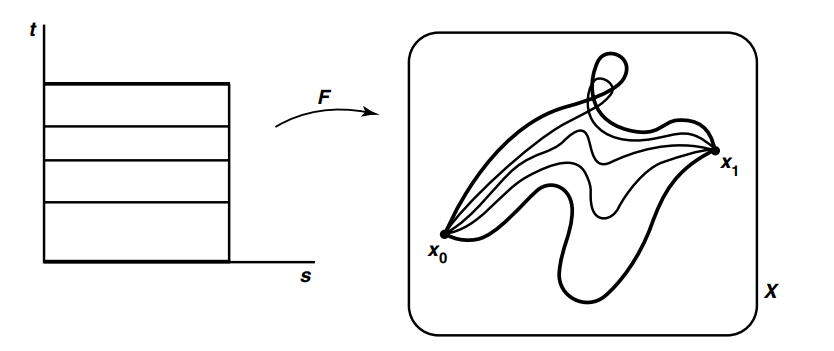
\includegraphics[width=0.5\linewidth]{Imagenes/imagen_2025-07-10_112455145.png}
    \end{figure}
\end{frame}
\begin{frame}
    \begin{block}{Definición}
        Dado $X$ espacio topologico y $x_0\in X$. El conjunto de clases de homotopia de caminos que inician y acaban en $x_0$, junto a la operacion de concatenar caminos lo llamamos el \textbf{grupo fundamental} de $X$ relativo a $x_0$ y que denotaremos por $\pi_1(X,x_0)$
        \end{block}

        \begin{block}{Definición}
        Un espacio topológico $X$ se dice \textbf{simplemente conexo} si es arco-conexo y su grupo fundamental es el trivial.
        \end{block}    
\end{frame}
\begin{frame}
    \begin{block}{Definición}
        Dado $X$ espacio topologico y $x_0\in X$. El conjunto de clases de homotopia de caminos que inician y acaban en $x_0$, junto a la operacion de concatenar caminos lo llamamos el \textbf{grupo fundamental} de $X$ relativo a $x_0$ y que denotaremos por $\pi_1(X,x_0)$
        \end{block}

        \begin{block}{Definición}
        Un espacio topológico $X$ se dice \textbf{simplemente conexo} si es arco-conexo y su grupo fundamental es el trivial.
        \end{block}    
\end{frame}
\begin{frame}
    \begin{block}{Definición}
        Sea $p:E\to B$ una función continua y sobreyectiva. Dado un abierto $U$ de $B$ se dice que esta cubierto uniformemente por $p$ is la imagen inversa de $U$ por $p$ puede ser escrita como unión de abiertos disyuntos $V_\alpha$ en $E$, y la restricción de $p$ a cada uno de estos es un homeomorfismo.
        \end{block} 
        \begin{figure}
            \centering
            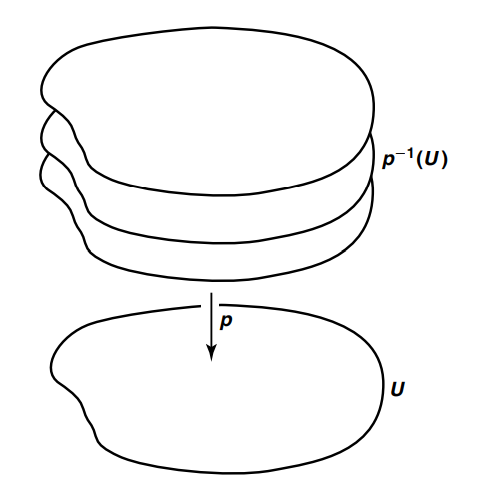
\includegraphics[width=0.4\linewidth]{Imagenes/imagen_2025-07-10_120527033.png}
        \end{figure}   
\end{frame}
\begin{frame}
        \begin{block}{Definición}
        Si para cada punto $b$ existe una vecindad $U$ tal que esta este cubuerta uniformemente se dice que $p$ es una funcion recubridora y que $E$ es el es \textbf{espacio recubridor}
        \end{block} 
        \begin{block}{Definición}
            Si el espacio recubridor $E$ es simplemente conexo se le llama el \textbf{cubrimiento universal}.
        \end{block}
        Al referirnos al cubrimiento universal de un espacio $X$ lo denotaremos por $\tilde{X}.$
        
\end{frame}
\begin{frame}{Teorema de Uniformizacion}
    \begin{block}{Teorema}
        Sea $X$ una superficie de Riemann simplemente conexa, entonces $X$ es biholomorfica a exactamente una de las siguientes superficies
        \begin{itemize}
            \item La esfera de Riemann $\C_{\infty}.$
            \item El plano Complejo $\C.$
            \item El semiplano superior $\Hs^2.$
        \end{itemize}
    \end{block}
    \textbf{Observación:} Note que a el cubrimiento universal lo podemos dotar de una estructura de superficie Riemann a partir de la de $X$, por lo que podemos pensar a las superficies de Riemann como cocientes de su cubrimiento universal.  
\end{frame}
\begin{frame}{Cocientes de superficies}
    En vista de lo anterior, lo natural seria pensar en las superficies de Riemann simplemente conexas y ver su posibles cocientes, pero resulta que para la esfera de Riemann y el plano complejo tenemos poca variedad
    \begin{block}{Proposicion}
        Sea $X$ una superficie de Riemann. El cubrimiento universal de $X$ es biholomorfo a $\C_\infty$ si y solo si $X$ es biholomorfo a $\C_\infty$
    \end{block}
    \begin{block}{Proposicion}
        Sea $X$ una superficie de Riemann. El cubrimiento universal de $X$ es biholomorfo a $\C$ si y solo si $X$ es biholomorfo a $\C,\C-\{0\}$ o $\C/L$
    \end{block}
    Resulta que donde tendremos una mayor variedad son los cocientes de $\Hs^2$, pero antes de ver esto estudiaremos
\end{frame}
\begin{frame}{Motivacion}

    Esto lo escribe el serco
    
\end{frame}
\begin{frame}{Aplicaciones conformes y cuasiconformes}
Sea $w=f(z)$ un homeomorfismo $C^1$ de una región a otra. En un punto $z_0$ se inducen aplicaciones lineales de diferenciales tal que
\begin{align*}
    du&=u_xdx+u_ydy,\\
    dv&=v_xdx+v_ydy.\\
\end{align*}
Donde $z=x+iy$ y $w=u+iv,$ Estos también se pueden ver de manera compleja pero concentremonos en que geometricamente  estos representan transfromaciones afines del plano $(dx,dy)$ al plano
$(du,dv).$\\

De esta manera estas transformaciones envían círculos centrados en el origen en elipses similares, es de nuestro interes ver la razón entre los ejes y como cambia su dirección.  
    
\end{frame}

\begin{frame}{}
    Aqui va lo de mapas conformes pero me raye
\end{frame}
\begin{frame}{Espacio de Teichmuller del Toro}
    En general un espacio de Teichmuller asociado a una superficie sera el espacio de de superficies de Riemann \textit{marcadas} de aquella superficie, mientras que el espacio de Moduli sera el de clases de isomorfismo de estas estructuras.\\
    \vspace{0.5cm}

    Por el Teorema de Uniformizacion solo podemos asignarle una estructura de superficie de Riemann a $\C_\infty$, por lo que segun nuestra idea general el espacio de Moduli es un único punto. Resulta que para el espacio de Teichmuller ocurre lo mismo, por lo que nuestro interés inicial sera estudiar estos espacios para los toros $\C/L$
\end{frame}
\begin{frame}{}
    Recordemos que los retículos están determinados por por una base de la forma $\{1,\tau\}$, donde $\tau\in \Hs^2$, 
\end{frame}




\begin{frame}{Referencias}

\end{frame}

\end{document}




